\section{IPI Protocol Design}
\label{sec:ipi}

A comparable evaluation of compact J2735 updates and correlated CAV operations
requires a workload representation that preserves existing J2735 content and
associates the requests, intermediate updates, and outcomes that belong to one
CAV operation. The Intersection Programming Interface (IPI) provides this
application-layer contract. It enables the measurement study and can also
support applications that use both workload classes.

\textbf{Application interface, wire protocol, runtime, and bindings.}
IPI comprises four components. First, the application programming interface
lets an application publish or receive a message, invoke an operation, retrieve
its responses, and manage an application session. Second, a
transport-independent wire protocol defines separate serialized profiles for
messages and operations. Third, the reference runtime validates frames and
maintains local session and response records. Fourth, a binding places each
serialized frame in PC5 custom data or an Internet Protocol transport on Uu.
Commonality resides in the application contract and operation semantics; each
profile serializes only the fields required by its workload and binding.

\textbf{Compact messages and correlated operations.}
The compact message profile carries an individual J2735 message. Typed helpers
cover Basic Safety Message (BSM), Personal Safety Message (PSM), Map Data (MAP),
Signal Phase and Timing (SPaT), Signal Request Message (SRM), and Signal Status
Message (SSM). The byte-preserving form wraps a complete pre-encoded J2735
message with a one-byte type and a four-byte length. It therefore retains the
deployed message bytes without adding operation state.

The correlated-operation profile represents perception, planning, control, and
map interactions. A request starts an operation. An update carries nonterminal
progress or intermediate content. A completion carries a successful terminal
result, and a rejection reports refusal or unsuccessful termination. The
correlation identifier associates each update or terminal result with its
request. The session identifier groups related operations within a continuing
interaction. Expiration identifies when an operation or result is no longer
useful. Registration establishes the application session, heartbeat refreshes
its lease, telemetry reports session-associated state, and termination closes
the session. An IPI application session is distinct from a Transmission Control
Protocol (TCP) connection, a Message Queuing Telemetry Transport (MQTT) session,
and a 3GPP protocol data unit or V2X Application Enabler session.

Typed planning, perception, and control content supports known objects. Opaque
content carries an application object together with its declared service class
when both endpoints use an external schema. Thus, the operation profile adds
the association and outcome fields required by stateful CAV interactions while
the compact profile leaves J2735 messages small.

\begin{table*}[t]
  \caption{IPI requirements, mechanisms, and supporting evidence.}
  \label{tab:ipi-design}
  \centering
  \footnotesize
  \setlength{\tabcolsep}{4pt}
  \renewcommand{\arraystretch}{1.10}
  \begin{tabular}{@{}p{0.20\textwidth}p{0.40\textwidth}p{0.31\textwidth}@{}}
    \toprule
    Requirement & IPI mechanism & Evidence in this paper \\
    \midrule
    Carry deployed CV/ITS messages & Typed helpers and byte-exact pre-encoded J2735 content & Callback, round-trip, and byte-preservation tests \\
    Represent a CAV operation lifecycle & Request, update, completion, rejection, session, correlation, and expiration fields & Lifecycle, correlation, and malformed-frame tests \\
    Use one application contract across paths & Distinct message/operation profiles and path-specific adapters behind one API & PC5 custom-data and Uu field campaigns \\
    Control representation size & Five-byte compact wrapper and bounded operation fields & Measured byte counts in Section~\ref{sec:results-functional} \\
    \bottomrule
  \end{tabular}
\end{table*}

\textbf{Responsibility boundary.}
IPI standardizes application representation, operation association, generic
outcome, and freshness. A binding supplies frame delimitation, datagram
formation, fragmentation and reassembly, delivery, retransmission, and
congestion behavior. The PC5 binding places one complete IPI frame in one
vendor custom-data payload. The TCP binding uses a four-byte network-order
length prefix. The MQTT binding places one serialized frame in one MQTT
application payload and uses Quality of Service (QoS)~0. Raw User Datagram
Protocol (UDP) places one frame in one
datagram when it fits; the
1,400-B fragmentation and reassembly evaluated later belong to the UDP
measurement adapter. The deployment configures security, admission, radio
scheduling, and path selection. The application determines
domain-specific decisions such as whether to accept a maneuver. These
responsibilities preserve application meaning while allowing communication behavior to
change across the paths evaluated in this paper.

Figure~\ref{fig:ipi-architecture} shows the resulting organization. The
application contract presents message and operation modes. Their serialized
profiles retain the compact or correlated fields needed by the selected PC5 or
Uu binding.

\begin{figure}[t]
  \centering
  \begin{tikzpicture}
    \node[inner sep=0] (ipiarch) {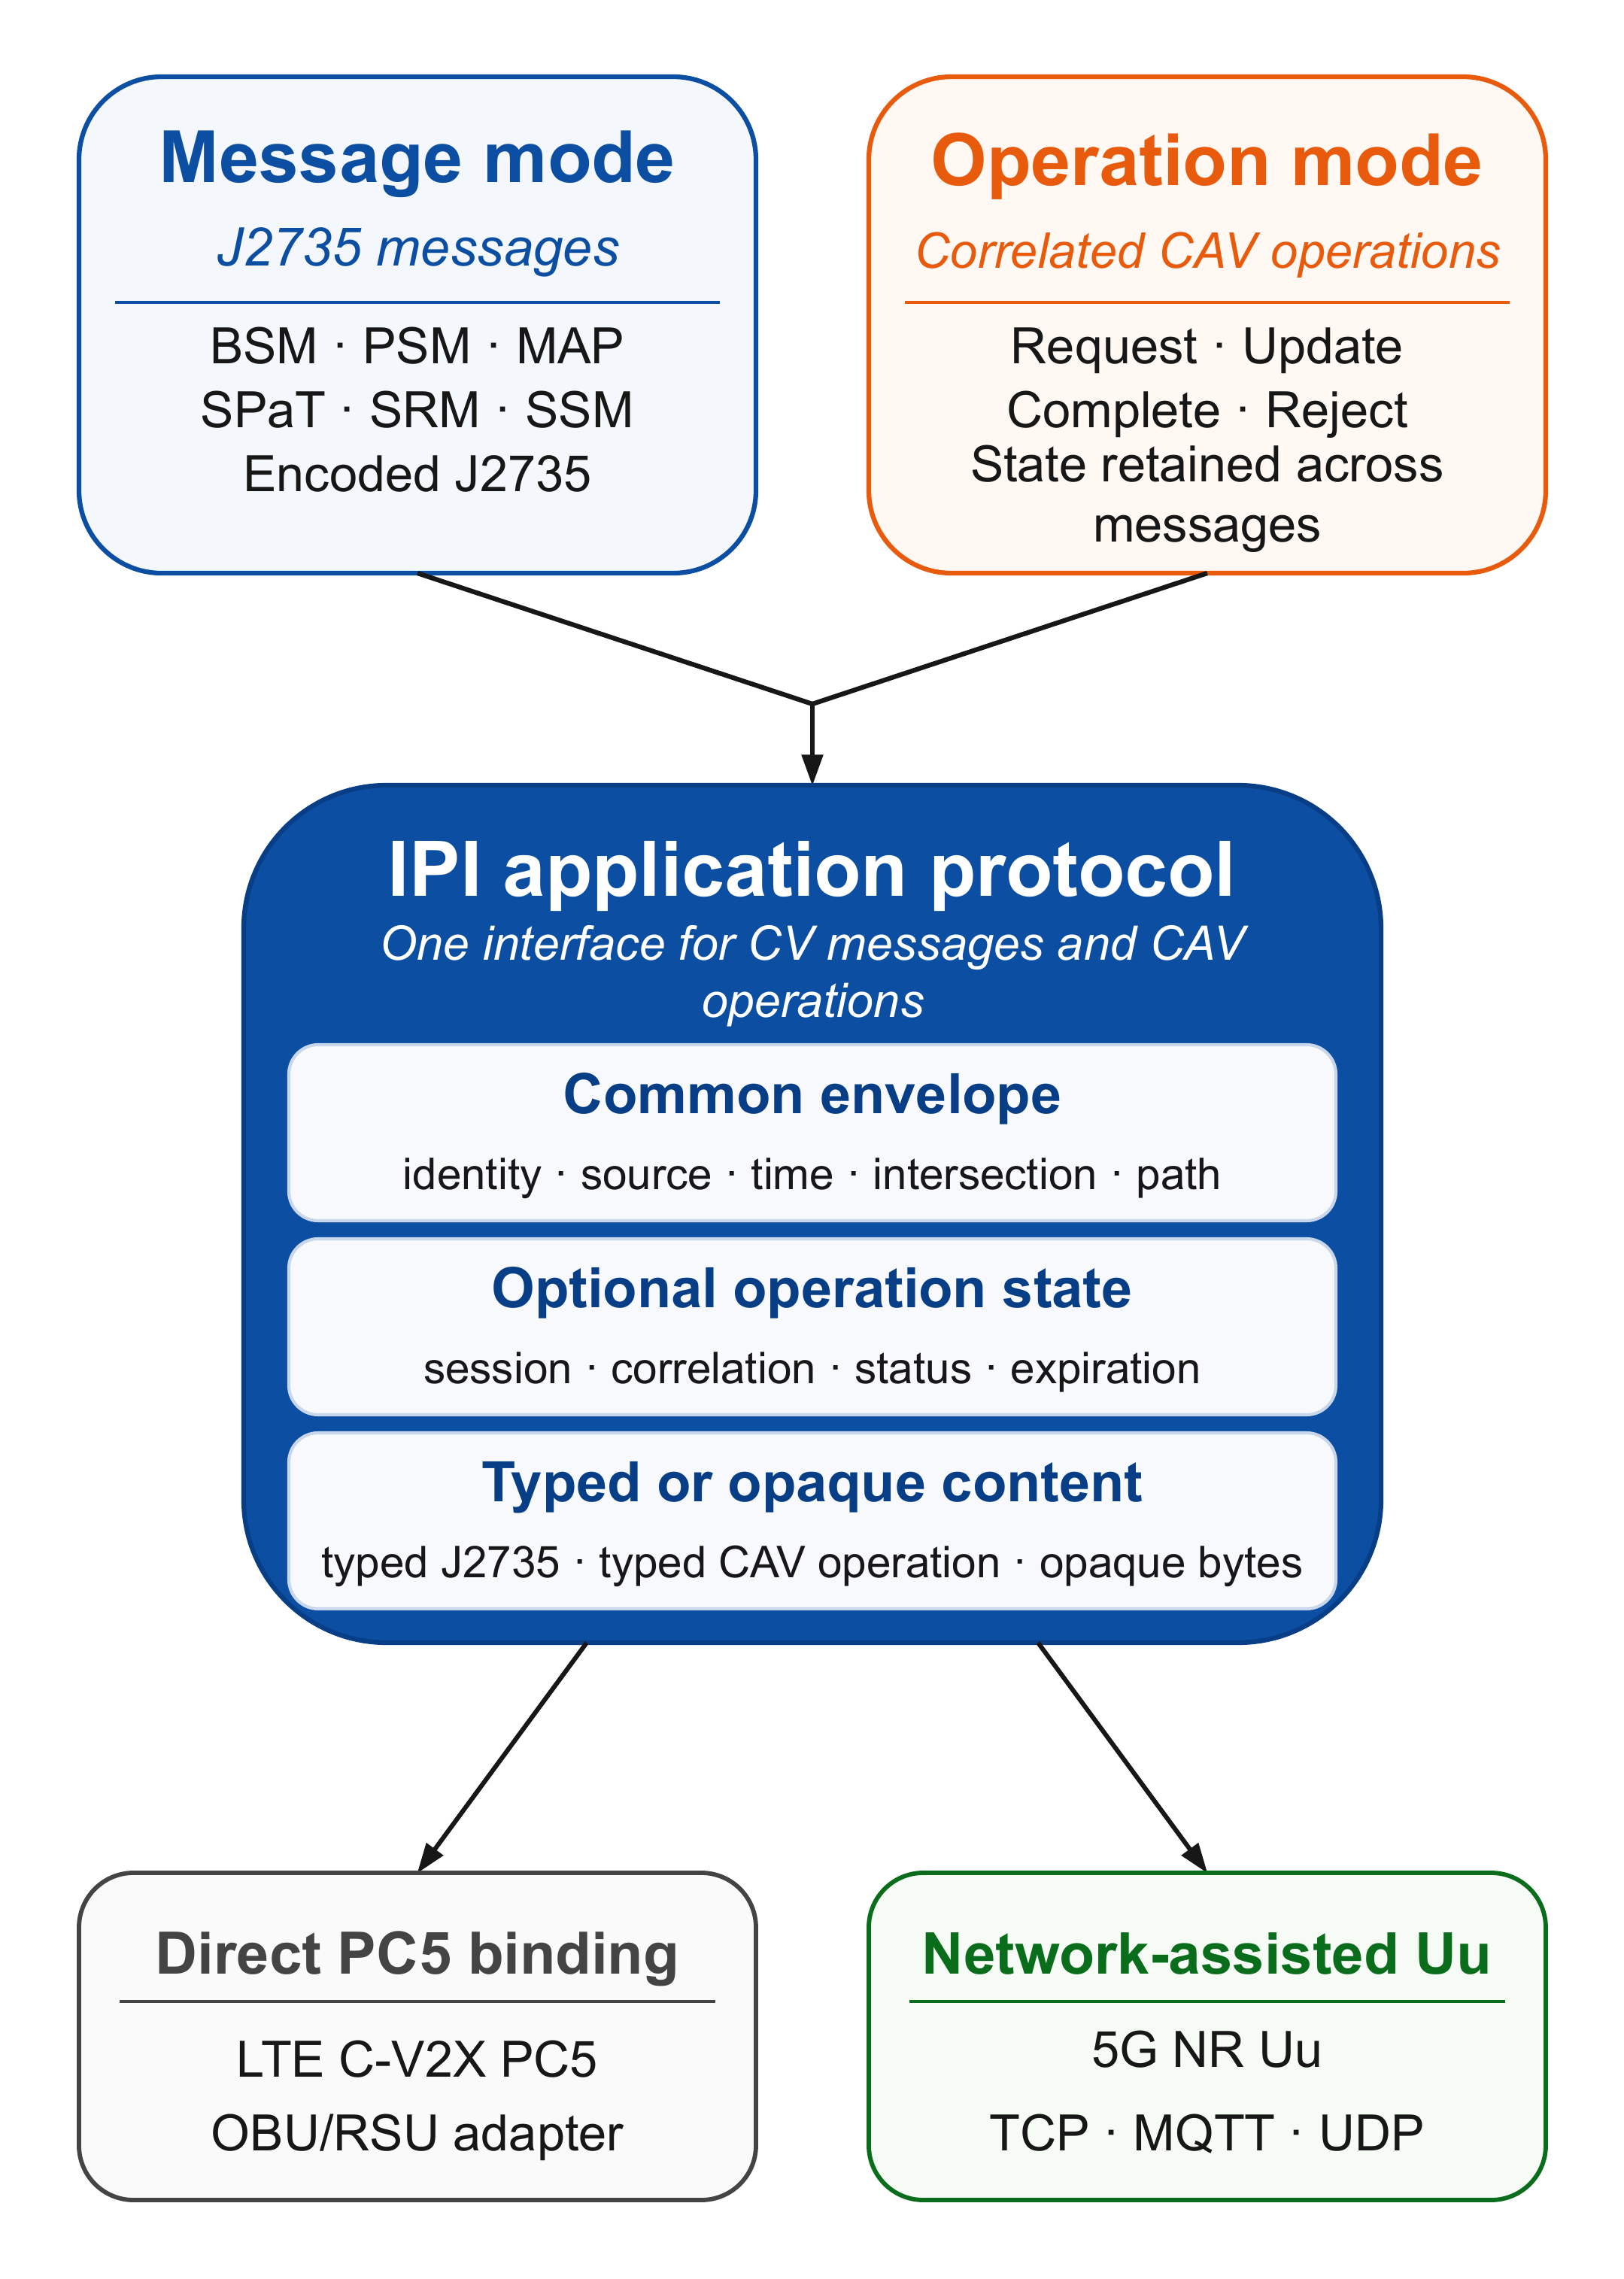
\includegraphics[width=\columnwidth]{figs/figure02_ipi_protocol_architecture_flat.png}};
    \node[fill=white,minimum width=0.72\columnwidth,minimum height=27pt]
      at (ipiarch.center) {};
    \node[text=blue!55!black,font=\sffamily\bfseries\small]
      at ([yshift=6pt]ipiarch.center) {Profile-selected metadata};
    \node[font=\sffamily\tiny]
      at ([yshift=-7pt]ipiarch.center)
      {compact: type, length \quad operation: identity, session, status};
  \end{tikzpicture}
  \caption{IPI presents one application contract for compact J2735 messages and
  correlated CAV operations. The compact and operation profiles use distinct
  serialized fields, and the selected binding carries the resulting frame over
  direct PC5 or network-assisted Uu.}
  \Description{J2735 message mode and correlated CAV operation mode enter one
  IPI application contract. The compact profile preserves typed or pre-encoded
  J2735 content, while the operation profile adds session, correlation, status,
  expiration, and typed or opaque CAV content. Path-specific bindings carry the
  resulting frames over direct PC5 or network-assisted Uu.}
  \label{fig:ipi-architecture}
\end{figure}

\textbf{Reference implementation.}
The C++17 implementation provides the four components above. Its tests exercise
typed and pre-encoded J2735 messages, independently generated J2735 IPI
conformance vectors, correlated operation roles, session lifecycle, malformed
input rejection, PC5 framing, and broker-backed operation exchange.
Section~\ref{sec:results-functional} measures the representation cost and
workload coverage. Section~\ref{sec:setup} next identifies the serialized IPI
profile and payload-size boundary used by each field campaign.
